\documentclass[]{book}
\usepackage{lmodern}
\usepackage{amssymb,amsmath}
\usepackage{ifxetex,ifluatex}
\usepackage{fixltx2e} % provides \textsubscript
\ifnum 0\ifxetex 1\fi\ifluatex 1\fi=0 % if pdftex
  \usepackage[T1]{fontenc}
  \usepackage[utf8]{inputenc}
\else % if luatex or xelatex
  \ifxetex
    \usepackage{mathspec}
  \else
    \usepackage{fontspec}
  \fi
  \defaultfontfeatures{Ligatures=TeX,Scale=MatchLowercase}
\fi
% use upquote if available, for straight quotes in verbatim environments
\IfFileExists{upquote.sty}{\usepackage{upquote}}{}
% use microtype if available
\IfFileExists{microtype.sty}{%
\usepackage[]{microtype}
\UseMicrotypeSet[protrusion]{basicmath} % disable protrusion for tt fonts
}{}
\PassOptionsToPackage{hyphens}{url} % url is loaded by hyperref
\usepackage[unicode=true]{hyperref}
\hypersetup{
            pdftitle={EVSC 3201 Materials},
            pdfauthor={Sean Hardison},
            pdfborder={0 0 0},
            breaklinks=true}
\urlstyle{same}  % don't use monospace font for urls
\usepackage{natbib}
\bibliographystyle{apalike}
\usepackage{color}
\usepackage{fancyvrb}
\newcommand{\VerbBar}{|}
\newcommand{\VERB}{\Verb[commandchars=\\\{\}]}
\DefineVerbatimEnvironment{Highlighting}{Verbatim}{commandchars=\\\{\}}
% Add ',fontsize=\small' for more characters per line
\usepackage{framed}
\definecolor{shadecolor}{RGB}{248,248,248}
\newenvironment{Shaded}{\begin{snugshade}}{\end{snugshade}}
\newcommand{\KeywordTok}[1]{\textcolor[rgb]{0.13,0.29,0.53}{\textbf{#1}}}
\newcommand{\DataTypeTok}[1]{\textcolor[rgb]{0.13,0.29,0.53}{#1}}
\newcommand{\DecValTok}[1]{\textcolor[rgb]{0.00,0.00,0.81}{#1}}
\newcommand{\BaseNTok}[1]{\textcolor[rgb]{0.00,0.00,0.81}{#1}}
\newcommand{\FloatTok}[1]{\textcolor[rgb]{0.00,0.00,0.81}{#1}}
\newcommand{\ConstantTok}[1]{\textcolor[rgb]{0.00,0.00,0.00}{#1}}
\newcommand{\CharTok}[1]{\textcolor[rgb]{0.31,0.60,0.02}{#1}}
\newcommand{\SpecialCharTok}[1]{\textcolor[rgb]{0.00,0.00,0.00}{#1}}
\newcommand{\StringTok}[1]{\textcolor[rgb]{0.31,0.60,0.02}{#1}}
\newcommand{\VerbatimStringTok}[1]{\textcolor[rgb]{0.31,0.60,0.02}{#1}}
\newcommand{\SpecialStringTok}[1]{\textcolor[rgb]{0.31,0.60,0.02}{#1}}
\newcommand{\ImportTok}[1]{#1}
\newcommand{\CommentTok}[1]{\textcolor[rgb]{0.56,0.35,0.01}{\textit{#1}}}
\newcommand{\DocumentationTok}[1]{\textcolor[rgb]{0.56,0.35,0.01}{\textbf{\textit{#1}}}}
\newcommand{\AnnotationTok}[1]{\textcolor[rgb]{0.56,0.35,0.01}{\textbf{\textit{#1}}}}
\newcommand{\CommentVarTok}[1]{\textcolor[rgb]{0.56,0.35,0.01}{\textbf{\textit{#1}}}}
\newcommand{\OtherTok}[1]{\textcolor[rgb]{0.56,0.35,0.01}{#1}}
\newcommand{\FunctionTok}[1]{\textcolor[rgb]{0.00,0.00,0.00}{#1}}
\newcommand{\VariableTok}[1]{\textcolor[rgb]{0.00,0.00,0.00}{#1}}
\newcommand{\ControlFlowTok}[1]{\textcolor[rgb]{0.13,0.29,0.53}{\textbf{#1}}}
\newcommand{\OperatorTok}[1]{\textcolor[rgb]{0.81,0.36,0.00}{\textbf{#1}}}
\newcommand{\BuiltInTok}[1]{#1}
\newcommand{\ExtensionTok}[1]{#1}
\newcommand{\PreprocessorTok}[1]{\textcolor[rgb]{0.56,0.35,0.01}{\textit{#1}}}
\newcommand{\AttributeTok}[1]{\textcolor[rgb]{0.77,0.63,0.00}{#1}}
\newcommand{\RegionMarkerTok}[1]{#1}
\newcommand{\InformationTok}[1]{\textcolor[rgb]{0.56,0.35,0.01}{\textbf{\textit{#1}}}}
\newcommand{\WarningTok}[1]{\textcolor[rgb]{0.56,0.35,0.01}{\textbf{\textit{#1}}}}
\newcommand{\AlertTok}[1]{\textcolor[rgb]{0.94,0.16,0.16}{#1}}
\newcommand{\ErrorTok}[1]{\textcolor[rgb]{0.64,0.00,0.00}{\textbf{#1}}}
\newcommand{\NormalTok}[1]{#1}
\usepackage{longtable,booktabs}
% Fix footnotes in tables (requires footnote package)
\IfFileExists{footnote.sty}{\usepackage{footnote}\makesavenoteenv{long table}}{}
\usepackage{graphicx,grffile}
\makeatletter
\def\maxwidth{\ifdim\Gin@nat@width>\linewidth\linewidth\else\Gin@nat@width\fi}
\def\maxheight{\ifdim\Gin@nat@height>\textheight\textheight\else\Gin@nat@height\fi}
\makeatother
% Scale images if necessary, so that they will not overflow the page
% margins by default, and it is still possible to overwrite the defaults
% using explicit options in \includegraphics[width, height, ...]{}
\setkeys{Gin}{width=\maxwidth,height=\maxheight,keepaspectratio}
\IfFileExists{parskip.sty}{%
\usepackage{parskip}
}{% else
\setlength{\parindent}{0pt}
\setlength{\parskip}{6pt plus 2pt minus 1pt}
}
\setlength{\emergencystretch}{3em}  % prevent overfull lines
\providecommand{\tightlist}{%
  \setlength{\itemsep}{0pt}\setlength{\parskip}{0pt}}
\setcounter{secnumdepth}{5}
% Redefines (sub)paragraphs to behave more like sections
\ifx\paragraph\undefined\else
\let\oldparagraph\paragraph
\renewcommand{\paragraph}[1]{\oldparagraph{#1}\mbox{}}
\fi
\ifx\subparagraph\undefined\else
\let\oldsubparagraph\subparagraph
\renewcommand{\subparagraph}[1]{\oldsubparagraph{#1}\mbox{}}
\fi

% set default figure placement to htbp
\makeatletter
\def\fps@figure{htbp}
\makeatother

\usepackage{booktabs}

\title{EVSC 3201 Materials}
\author{Sean Hardison}
\date{2020-07-15}

\begin{document}
\maketitle

{
\setcounter{tocdepth}{1}
\tableofcontents
}
\chapter*{Introduction}\label{introduction}
\addcontentsline{toc}{chapter}{Introduction}

In light of the extenuating circumstances regarding COVID-19, I've
decided to experiment with a new format for teaching the Fundamental of
Ecology Lab. For the rest of the semester, I'll add instructions, notes,
and videos to tabs on this site. The goal of these materials is to
supplement the lab manual by providing some interactivity that we're
missing out on by not meeting face-to-face. Assignments due each week
will be added to the bottom of each page.

\chapter{Forest Lab Data Analysis:
Results}\label{forest-lab-data-analysis-results}

See below for results from the forest lab field study. When answering
the questions on page 27 of your lab manual, make sure your
interpretations align with what's shown here.

\section{Processing and analytical
code}\label{processing-and-analytical-code}

\textbf{Important}: This code must be evaluated prior to running any
other code in this document. Note that I used \texttt{read\_excel} to
read in data directly from where it is located on my computer. To
reproduce these analyses you will need to alter those lines to match
where the data is located on your own computer.

\begin{Shaded}
\begin{Highlighting}[]
\CommentTok{# read in libraries}
\KeywordTok{library}\NormalTok{(readxl)}
\KeywordTok{library}\NormalTok{(tidyverse)}


\CommentTok{#read in data - change these lines to reflect where the data are stored on your computer}
\NormalTok{env =}\StringTok{ }\KeywordTok{read_excel}\NormalTok{(}\StringTok{"/users/seanhardison/desktop/ecology lab/environmental_data.xlsx"}\NormalTok{)}
\NormalTok{forest =}\StringTok{ }\KeywordTok{read_excel}\NormalTok{(}\StringTok{"/users/seanhardison/desktop/ecology lab/forest_lab.xlsx"}\NormalTok{)}

\CommentTok{#summarise data}
\NormalTok{summary_env =}\StringTok{ }\NormalTok{env }\OperatorTok\StringTok{ }
\StringTok{  }
\StringTok{  }\CommentTok{#create new column for slope angle}
\StringTok{  }\KeywordTok{mutate}\NormalTok{(}\DataTypeTok{slope_angle =} \KeywordTok{atan}\NormalTok{(Rise}\OperatorTok{/}\NormalTok{Run) }\OperatorTok{*}\StringTok{ }\DecValTok{180}\OperatorTok{/}\NormalTok{pi) }\OperatorTok\StringTok{ }
\StringTok{  }
\StringTok{  }\CommentTok{#Tell R to group by Site for finding mean and standard deviation}
\StringTok{  }\KeywordTok{group_by}\NormalTok{(Site) }\OperatorTok\StringTok{ }
\StringTok{  }
\StringTok{  }\CommentTok{#Find the mean and standard deviation by site}
\StringTok{  }\KeywordTok{summarise}\NormalTok{(}\DataTypeTok{mean_slope_angle =} \KeywordTok{mean}\NormalTok{(slope_angle, }\DataTypeTok{na.rm =}\NormalTok{ T),}
            \DataTypeTok{sd_slope_angle =} \KeywordTok{sd}\NormalTok{(slope_angle, }\DataTypeTok{na.rm =}\NormalTok{ T),}
            
            \DataTypeTok{mean_thickness =} \KeywordTok{mean}\NormalTok{(}\StringTok{`}\DataTypeTok{Horizon Thickness}\StringTok{`}\NormalTok{),}
            \DataTypeTok{sd_thickness =} \KeywordTok{sd}\NormalTok{(}\StringTok{`}\DataTypeTok{Horizon Thickness}\StringTok{`}\NormalTok{),}
            
            \DataTypeTok{mean_moisture =} \KeywordTok{mean}\NormalTok{(}\StringTok{`}\DataTypeTok{Soil Moisture}\StringTok{`}\NormalTok{),}
            \DataTypeTok{sd_moisture =} \KeywordTok{sd}\NormalTok{(}\StringTok{`}\DataTypeTok{Soil Moisture}\StringTok{`}\NormalTok{),}
            
            \DataTypeTok{mean_temperature =} \KeywordTok{mean}\NormalTok{(}\StringTok{`}\DataTypeTok{Soil Temperature}\StringTok{`}\NormalTok{),}
            \DataTypeTok{sd_temperature =} \KeywordTok{sd}\NormalTok{(}\StringTok{`}\DataTypeTok{Soil Temperature}\StringTok{`}\NormalTok{))}
\end{Highlighting}
\end{Shaded}

\section{Environmental data: barplots
(Q1)}\label{environmental-data-barplots-q1}

\subsection*{Slope angle}\label{slope-angle}
\addcontentsline{toc}{subsection}{Slope angle}

\begin{Shaded}
\begin{Highlighting}[]
\KeywordTok{ggplot}\NormalTok{(summary_env) }\OperatorTok{+}
\StringTok{  }\KeywordTok{geom_bar}\NormalTok{(}\KeywordTok{aes}\NormalTok{(}\DataTypeTok{x =}\NormalTok{ Site, }\DataTypeTok{y =}\NormalTok{ mean_slope_angle), }\DataTypeTok{stat =} \StringTok{"identity"}\NormalTok{) }\OperatorTok{+}
\StringTok{  }\KeywordTok{geom_errorbar}\NormalTok{(}\KeywordTok{aes}\NormalTok{(}\DataTypeTok{x =}\NormalTok{ Site, }\DataTypeTok{ymin =}\NormalTok{ mean_slope_angle }\OperatorTok{-}\StringTok{ }\NormalTok{sd_slope_angle, }
                    \DataTypeTok{ymax =}\NormalTok{ mean_slope_angle }\OperatorTok{+}\StringTok{ }\NormalTok{sd_slope_angle),}
                \DataTypeTok{width =} \FloatTok{0.25}\NormalTok{) }\OperatorTok{+}
\StringTok{  }\KeywordTok{ylab}\NormalTok{(}\StringTok{"Mean slope angle (°)"}\NormalTok{) }\OperatorTok{+}
\StringTok{  }\KeywordTok{theme_bw}\NormalTok{()}
\end{Highlighting}
\end{Shaded}

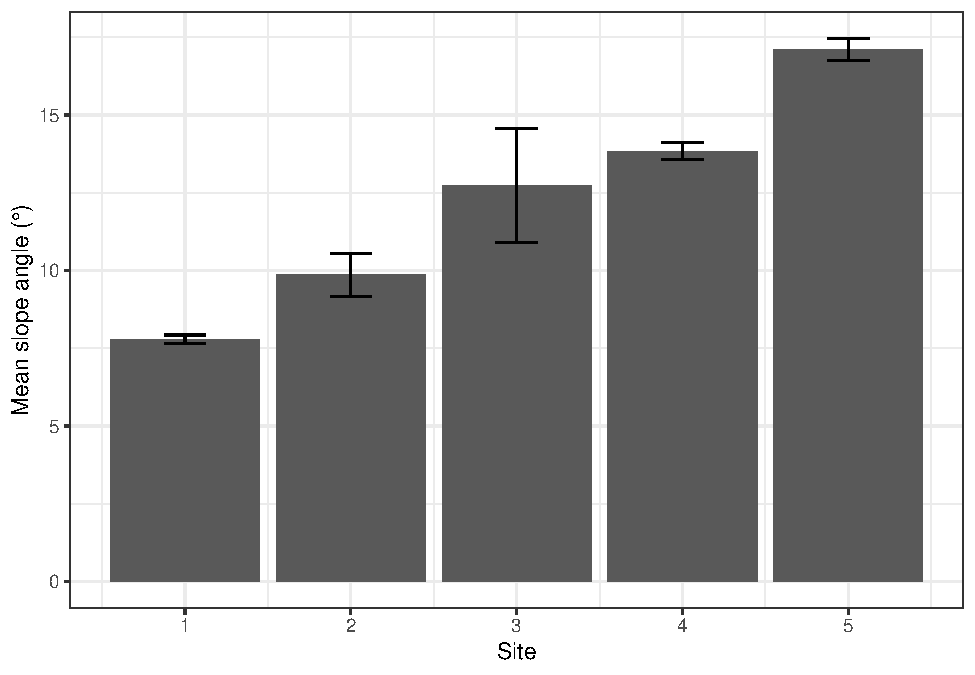
\includegraphics{EVCS-3201_files/figure-latex/unnamed-chunk-3-1.pdf}

\subsection*{Horizon thickness}\label{horizon-thickness}
\addcontentsline{toc}{subsection}{Horizon thickness}

\begin{Shaded}
\begin{Highlighting}[]
\KeywordTok{ggplot}\NormalTok{(summary_env) }\OperatorTok{+}
\StringTok{  }\KeywordTok{geom_bar}\NormalTok{(}\KeywordTok{aes}\NormalTok{(}\DataTypeTok{x =}\NormalTok{ Site, }\DataTypeTok{y =}\NormalTok{ mean_thickness), }\DataTypeTok{stat =} \StringTok{"identity"}\NormalTok{) }\OperatorTok{+}
\StringTok{  }\KeywordTok{geom_errorbar}\NormalTok{(}\KeywordTok{aes}\NormalTok{(}\DataTypeTok{x =}\NormalTok{ Site, }\DataTypeTok{ymin =}\NormalTok{ mean_thickness }\OperatorTok{-}\StringTok{ }\NormalTok{sd_thickness, }
                    \DataTypeTok{ymax =}\NormalTok{ mean_thickness }\OperatorTok{+}\StringTok{ }\NormalTok{sd_thickness),}
                \DataTypeTok{width =} \FloatTok{0.25}\NormalTok{) }\OperatorTok{+}
\StringTok{  }\KeywordTok{ylab}\NormalTok{(}\StringTok{"Mean horizon thickness (cm)"}\NormalTok{) }\OperatorTok{+}
\StringTok{  }\KeywordTok{theme_bw}\NormalTok{()}
\end{Highlighting}
\end{Shaded}

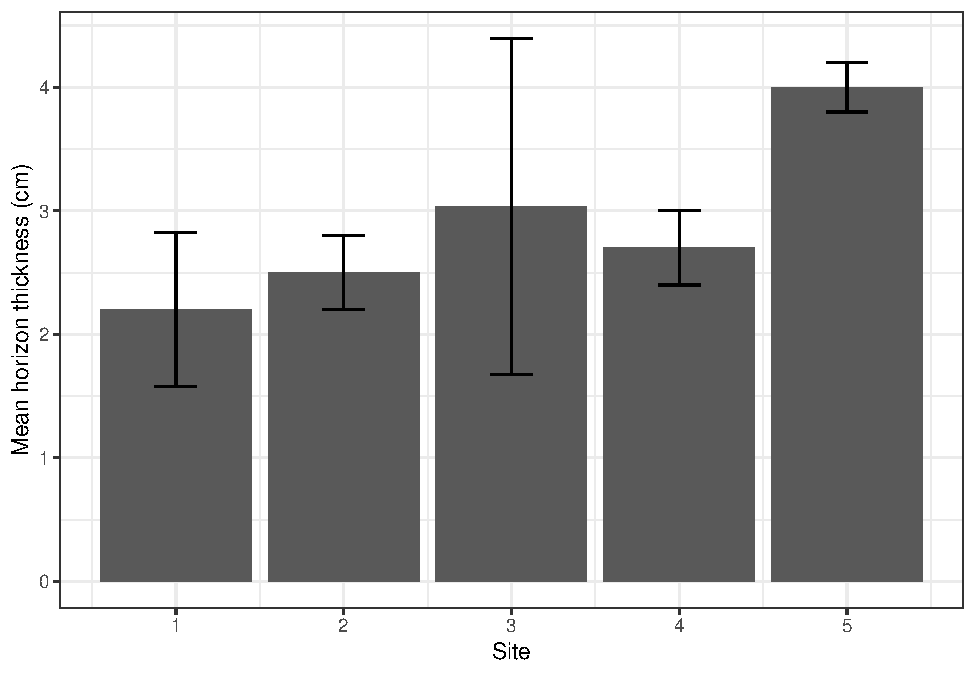
\includegraphics{EVCS-3201_files/figure-latex/unnamed-chunk-4-1.pdf}

\subsection*{Soil temperature}\label{soil-temperature}
\addcontentsline{toc}{subsection}{Soil temperature}

\begin{Shaded}
\begin{Highlighting}[]
\KeywordTok{ggplot}\NormalTok{(summary_env) }\OperatorTok{+}
\StringTok{  }\KeywordTok{geom_bar}\NormalTok{(}\KeywordTok{aes}\NormalTok{(}\DataTypeTok{x =}\NormalTok{ Site, }\DataTypeTok{y =}\NormalTok{ mean_temperature), }\DataTypeTok{stat =} \StringTok{"identity"}\NormalTok{) }\OperatorTok{+}
\StringTok{  }\KeywordTok{geom_errorbar}\NormalTok{(}\KeywordTok{aes}\NormalTok{(}\DataTypeTok{x =}\NormalTok{ Site, }\DataTypeTok{ymin =}\NormalTok{ mean_temperature }\OperatorTok{-}\StringTok{ }\NormalTok{sd_temperature, }
                    \DataTypeTok{ymax =}\NormalTok{ mean_temperature }\OperatorTok{+}\StringTok{ }\NormalTok{sd_temperature),}
                \DataTypeTok{width =} \FloatTok{0.25}\NormalTok{) }\OperatorTok{+}
\StringTok{  }\KeywordTok{ylab}\NormalTok{(}\StringTok{"Mean soil temperature (°F)"}\NormalTok{) }\OperatorTok{+}
\StringTok{  }\KeywordTok{theme_bw}\NormalTok{()}
\end{Highlighting}
\end{Shaded}

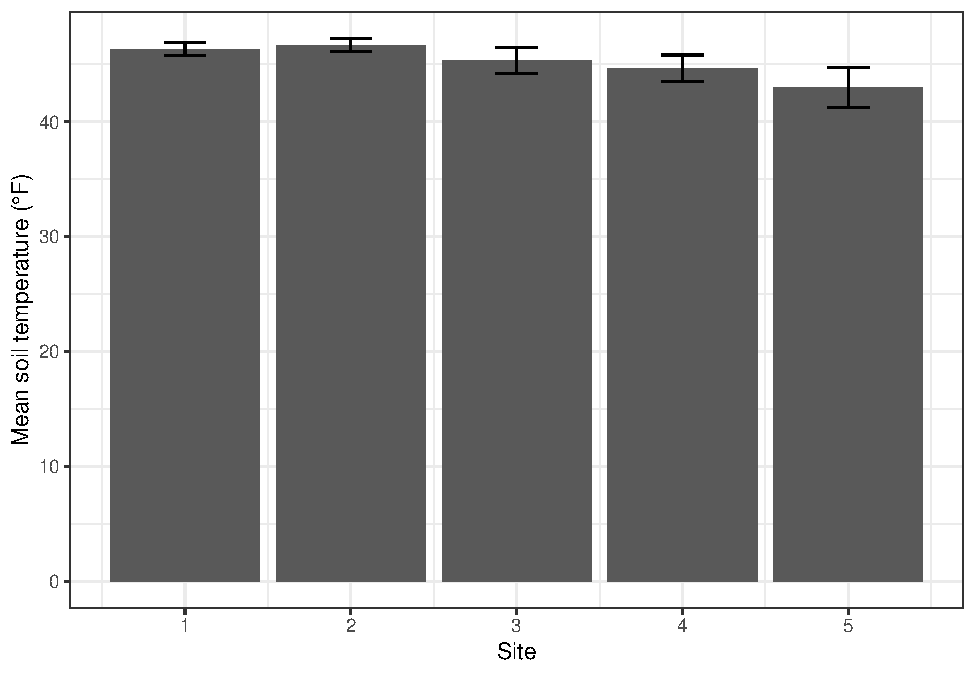
\includegraphics{EVCS-3201_files/figure-latex/unnamed-chunk-5-1.pdf}

\subsection*{Soil moisture}\label{soil-moisture}
\addcontentsline{toc}{subsection}{Soil moisture}

\begin{Shaded}
\begin{Highlighting}[]
\KeywordTok{ggplot}\NormalTok{(summary_env) }\OperatorTok{+}
\StringTok{  }\KeywordTok{geom_bar}\NormalTok{(}\KeywordTok{aes}\NormalTok{(}\DataTypeTok{x =}\NormalTok{ Site, }\DataTypeTok{y =}\NormalTok{ mean_moisture), }\DataTypeTok{stat =} \StringTok{"identity"}\NormalTok{) }\OperatorTok{+}
\StringTok{  }\KeywordTok{geom_errorbar}\NormalTok{(}\KeywordTok{aes}\NormalTok{(}\DataTypeTok{x =}\NormalTok{ Site, }\DataTypeTok{ymin =}\NormalTok{ mean_moisture }\OperatorTok{-}\StringTok{ }\NormalTok{sd_moisture, }
                    \DataTypeTok{ymax =}\NormalTok{ mean_moisture }\OperatorTok{+}\StringTok{ }\NormalTok{sd_moisture),}
                \DataTypeTok{width =} \FloatTok{0.25}\NormalTok{) }\OperatorTok{+}
\StringTok{  }\KeywordTok{ylab}\NormalTok{(}\StringTok{"Mean soil moisture (%)"}\NormalTok{) }\OperatorTok{+}
\StringTok{  }\KeywordTok{theme_bw}\NormalTok{()}
\end{Highlighting}
\end{Shaded}

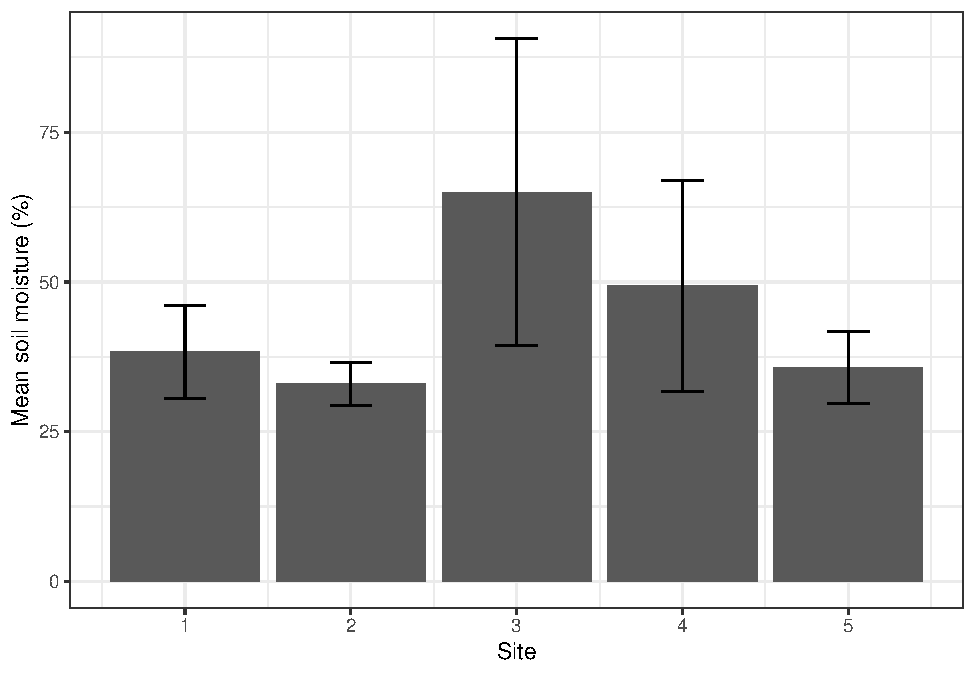
\includegraphics{EVCS-3201_files/figure-latex/unnamed-chunk-6-1.pdf}

\section{Environmental data: linear models and scatter plots
(Q2)}\label{environmental-data-linear-models-and-scatter-plots-q2}

Lines of best fit are shown on plots when significant relationships (P
\textless{} 0.05) are identified using linear models.

\subsection*{soil temperature \textasciitilde{} soil
moisture}\label{soil-temperature-soil-moisture}
\addcontentsline{toc}{subsection}{soil temperature \textasciitilde{}
soil moisture}

\begin{Shaded}
\begin{Highlighting}[]
\KeywordTok{ggplot}\NormalTok{(summary_env) }\OperatorTok{+}
\StringTok{  }\KeywordTok{geom_point}\NormalTok{(}\KeywordTok{aes}\NormalTok{(}\DataTypeTok{x =}\NormalTok{ mean_moisture, }\DataTypeTok{y =}\NormalTok{ mean_temperature)) }\OperatorTok{+}
\StringTok{  }\KeywordTok{ylab}\NormalTok{(}\StringTok{"Mean temperature (°F)"}\NormalTok{) }\OperatorTok{+}
\StringTok{  }\KeywordTok{xlab}\NormalTok{(}\StringTok{"Mean soil moisture (%)"}\NormalTok{)}
\end{Highlighting}
\end{Shaded}

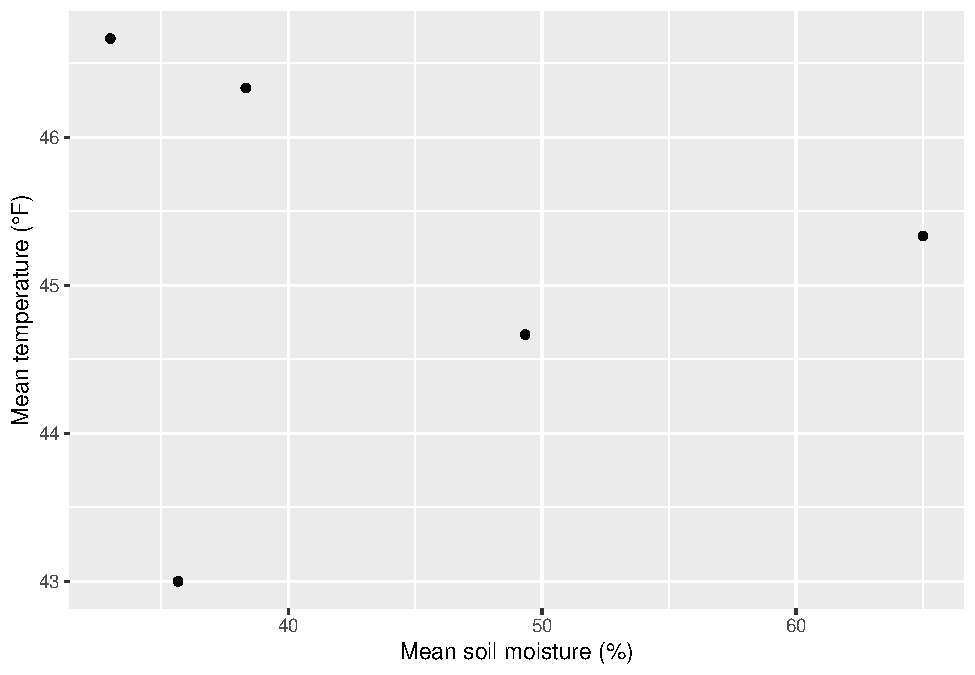
\includegraphics{EVCS-3201_files/figure-latex/unnamed-chunk-7-1.pdf}

\begin{Shaded}
\begin{Highlighting}[]
\NormalTok{temp_moisture_mod =}\StringTok{ }\KeywordTok{lm}\NormalTok{(mean_temperature }\OperatorTok{~}\StringTok{ }\NormalTok{mean_moisture, }\DataTypeTok{data =}\NormalTok{ summary_env)}
\KeywordTok{summary}\NormalTok{(temp_moisture_mod)}
\end{Highlighting}
\end{Shaded}

\begin{verbatim}
## 
## Call:
## lm(formula = mean_temperature ~ mean_moisture, data = summary_env)
## 
## Residuals:
##       1       2       3       4       5 
##  1.0967  1.3972  0.2612 -0.5021 -2.2531 
## 
## Coefficients:
##                Estimate Std. Error t value Pr(>|t|)    
## (Intercept)   45.473075   2.940404  15.465 0.000587 ***
## mean_moisture -0.006169   0.064197  -0.096 0.929507    
## ---
## Signif. codes:  0 '***' 0.001 '**' 0.01 '*' 0.05 '.' 0.1 ' ' 1
## 
## Residual standard error: 1.688 on 3 degrees of freedom
## Multiple R-squared:  0.003068,   Adjusted R-squared:  -0.3292 
## F-statistic: 0.009234 on 1 and 3 DF,  p-value: 0.9295
\end{verbatim}

\subsection*{soil moisture \textasciitilde{} horizon
thickness}\label{soil-moisture-horizon-thickness}
\addcontentsline{toc}{subsection}{soil moisture \textasciitilde{}
horizon thickness}

\begin{Shaded}
\begin{Highlighting}[]
\KeywordTok{ggplot}\NormalTok{(summary_env) }\OperatorTok{+}
\StringTok{  }\KeywordTok{geom_point}\NormalTok{(}\KeywordTok{aes}\NormalTok{(}\DataTypeTok{x =}\NormalTok{ mean_thickness, }\DataTypeTok{y =}\NormalTok{ mean_moisture)) }\OperatorTok{+}
\StringTok{  }\KeywordTok{ylab}\NormalTok{(}\StringTok{"Mean temperature (°F)"}\NormalTok{) }\OperatorTok{+}
\StringTok{  }\KeywordTok{xlab}\NormalTok{(}\StringTok{"Mean horizon thickness (cm)"}\NormalTok{)}
\end{Highlighting}
\end{Shaded}

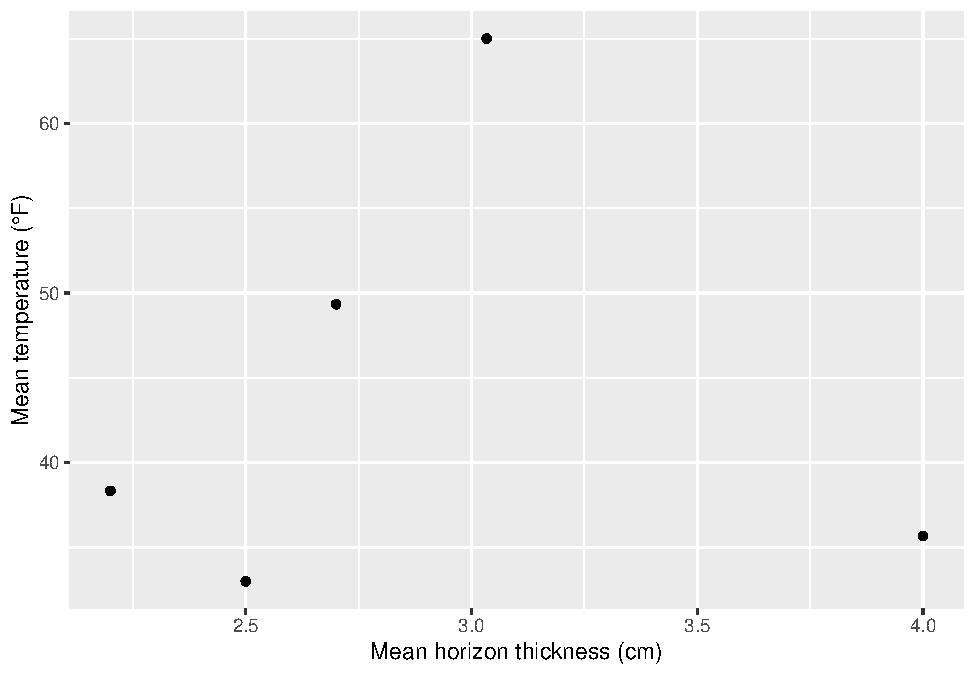
\includegraphics{EVCS-3201_files/figure-latex/unnamed-chunk-8-1.pdf}

\begin{Shaded}
\begin{Highlighting}[]
\NormalTok{moist_hor_thickness_mod =}\StringTok{ }\KeywordTok{lm}\NormalTok{(mean_moisture }\OperatorTok{~}\StringTok{ }\NormalTok{mean_thickness, }\DataTypeTok{data =}\NormalTok{ summary_env)}
\KeywordTok{summary}\NormalTok{(moist_hor_thickness_mod)}
\end{Highlighting}
\end{Shaded}

\begin{verbatim}
## 
## Call:
## lm(formula = mean_moisture ~ mean_thickness, data = summary_env)
## 
## Residuals:
##       1       2       3       4       5 
##  -5.593 -11.075  20.661   5.159  -9.152 
## 
## Coefficients:
##                Estimate Std. Error t value Pr(>|t|)
## (Intercept)     42.8344    32.3667   1.323    0.278
## mean_thickness   0.4962    10.9631   0.045    0.967
## 
## Residual standard error: 15.18 on 3 degrees of freedom
## Multiple R-squared:  0.0006823,  Adjusted R-squared:  -0.3324 
## F-statistic: 0.002048 on 1 and 3 DF,  p-value: 0.9667
\end{verbatim}

\subsection*{soil temperature \textasciitilde{} horizon
thickness}\label{soil-temperature-horizon-thickness}
\addcontentsline{toc}{subsection}{soil temperature \textasciitilde{}
horizon thickness}

\begin{Shaded}
\begin{Highlighting}[]
\KeywordTok{ggplot}\NormalTok{(summary_env) }\OperatorTok{+}
\StringTok{  }\KeywordTok{geom_point}\NormalTok{(}\KeywordTok{aes}\NormalTok{(}\DataTypeTok{x =}\NormalTok{ mean_thickness, }\DataTypeTok{y =}\NormalTok{ mean_temperature)) }\OperatorTok{+}
\StringTok{  }\KeywordTok{ylab}\NormalTok{(}\StringTok{"Mean temperature (°F)"}\NormalTok{) }\OperatorTok{+}
\StringTok{  }\KeywordTok{xlab}\NormalTok{(}\StringTok{"Mean horizon thickness (cm)"}\NormalTok{) }\OperatorTok{+}
\StringTok{  }\KeywordTok{geom_smooth}\NormalTok{(}\KeywordTok{aes}\NormalTok{(}\DataTypeTok{x =}\NormalTok{ mean_thickness, }\DataTypeTok{y =}\NormalTok{ mean_temperature), }\DataTypeTok{method =} \StringTok{"lm"}\NormalTok{)}
\end{Highlighting}
\end{Shaded}

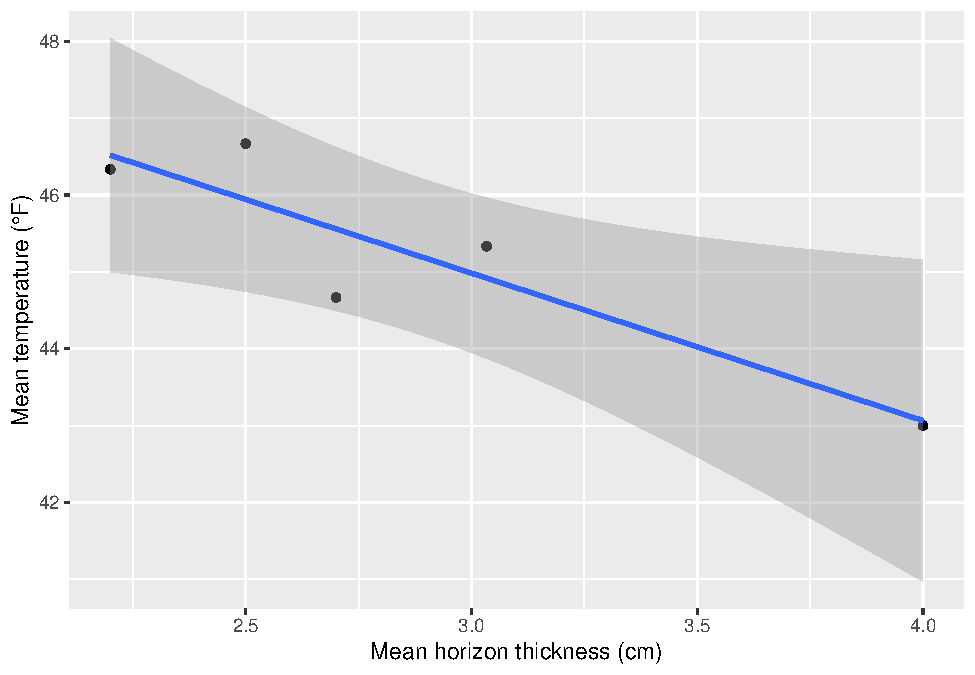
\includegraphics{EVCS-3201_files/figure-latex/unnamed-chunk-9-1.pdf}

\begin{Shaded}
\begin{Highlighting}[]
\NormalTok{temp_thick_mod =}\StringTok{ }\KeywordTok{lm}\NormalTok{(mean_temperature }\OperatorTok{~}\StringTok{ }\NormalTok{mean_thickness, }\DataTypeTok{data =}\NormalTok{ summary_env)}
\KeywordTok{summary}\NormalTok{(temp_thick_mod)}
\end{Highlighting}
\end{Shaded}

\begin{verbatim}
## 
## Call:
## lm(formula = mean_temperature ~ mean_thickness, data = summary_env)
## 
## Residuals:
##        1        2        3        4        5 
## -0.18332  0.72525  0.41456 -0.89126 -0.06523 
## 
## Coefficients:
##                Estimate Std. Error t value Pr(>|t|)    
## (Intercept)     50.7351     1.5229  33.316 5.94e-05 ***
## mean_thickness  -1.9175     0.5158  -3.717   0.0339 *  
## ---
## Signif. codes:  0 '***' 0.001 '**' 0.01 '*' 0.05 '.' 0.1 ' ' 1
## 
## Residual standard error: 0.7142 on 3 degrees of freedom
## Multiple R-squared:  0.8216, Adjusted R-squared:  0.7622 
## F-statistic: 13.82 on 1 and 3 DF,  p-value: 0.03387
\end{verbatim}

\subsection*{horizon thickness \textasciitilde{} slope
angle}\label{horizon-thickness-slope-angle}
\addcontentsline{toc}{subsection}{horizon thickness \textasciitilde{}
slope angle}

\begin{Shaded}
\begin{Highlighting}[]
\KeywordTok{ggplot}\NormalTok{(summary_env) }\OperatorTok{+}
\StringTok{  }\KeywordTok{geom_point}\NormalTok{(}\KeywordTok{aes}\NormalTok{(}\DataTypeTok{x =}\NormalTok{ mean_slope_angle, }\DataTypeTok{y =}\NormalTok{ mean_thickness)) }\OperatorTok{+}
\StringTok{  }\KeywordTok{ylab}\NormalTok{(}\StringTok{"Mean horizon thickness (cm)"}\NormalTok{) }\OperatorTok{+}
\StringTok{  }\KeywordTok{xlab}\NormalTok{(}\StringTok{"Mean slope angle (°)"}\NormalTok{) }\OperatorTok{+}
\StringTok{  }\KeywordTok{geom_smooth}\NormalTok{(}\KeywordTok{aes}\NormalTok{(}\DataTypeTok{x =}\NormalTok{ mean_slope_angle, }\DataTypeTok{y =}\NormalTok{ mean_thickness), }\DataTypeTok{method =} \StringTok{"lm"}\NormalTok{)}
\end{Highlighting}
\end{Shaded}

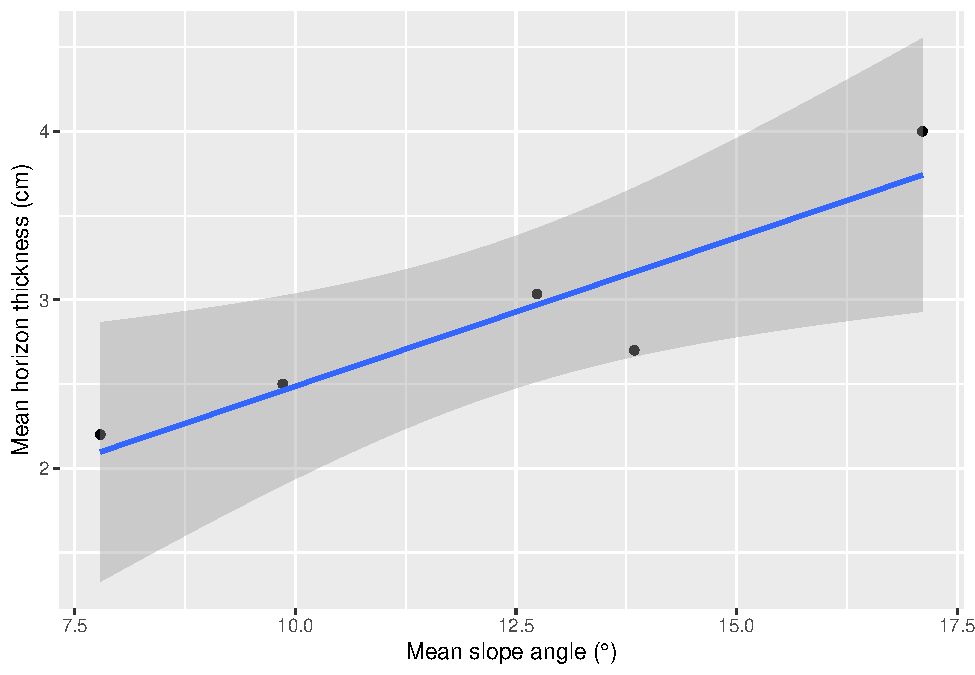
\includegraphics{EVCS-3201_files/figure-latex/unnamed-chunk-10-1.pdf}

\begin{Shaded}
\begin{Highlighting}[]
\NormalTok{thickness_slope_mod =}\StringTok{ }\KeywordTok{lm}\NormalTok{(mean_thickness }\OperatorTok{~}\StringTok{ }\NormalTok{mean_slope_angle, }\DataTypeTok{data =}\NormalTok{ summary_env)}
\KeywordTok{summary}\NormalTok{(thickness_slope_mod)}
\end{Highlighting}
\end{Shaded}

\begin{verbatim}
## 
## Call:
## lm(formula = mean_thickness ~ mean_slope_angle, data = summary_env)
## 
## Residuals:
##        1        2        3        4        5 
##  0.10310  0.03869  0.06312 -0.46425  0.25934 
## 
## Coefficients:
##                  Estimate Std. Error t value Pr(>|t|)  
## (Intercept)       0.72216    0.55535    1.30   0.2844  
## mean_slope_angle  0.17646    0.04379    4.03   0.0275 *
## ---
## Signif. codes:  0 '***' 0.001 '**' 0.01 '*' 0.05 '.' 0.1 ' ' 1
## 
## Residual standard error: 0.3156 on 3 degrees of freedom
## Multiple R-squared:  0.8441, Adjusted R-squared:  0.7921 
## F-statistic: 16.24 on 1 and 3 DF,  p-value: 0.02747
\end{verbatim}

\subsection*{soil moisture \textasciitilde{} slope
angle}\label{soil-moisture-slope-angle}
\addcontentsline{toc}{subsection}{soil moisture \textasciitilde{} slope
angle}

\begin{Shaded}
\begin{Highlighting}[]
\KeywordTok{ggplot}\NormalTok{(summary_env) }\OperatorTok{+}
\StringTok{  }\KeywordTok{geom_point}\NormalTok{(}\KeywordTok{aes}\NormalTok{(}\DataTypeTok{x =}\NormalTok{ mean_slope_angle, }\DataTypeTok{y =}\NormalTok{ mean_moisture)) }\OperatorTok{+}
\StringTok{  }\KeywordTok{ylab}\NormalTok{(}\StringTok{"Mean soil moisture (%)"}\NormalTok{) }\OperatorTok{+}
\StringTok{  }\KeywordTok{xlab}\NormalTok{(}\StringTok{"Mean slope angle (°)"}\NormalTok{) }
\end{Highlighting}
\end{Shaded}

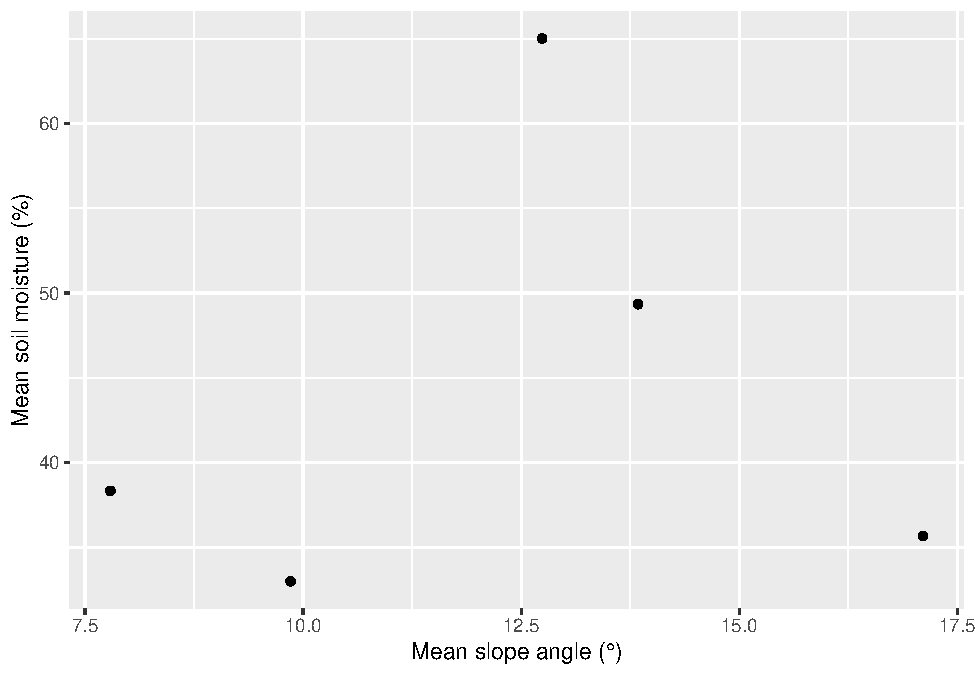
\includegraphics{EVCS-3201_files/figure-latex/unnamed-chunk-11-1.pdf}

\begin{Shaded}
\begin{Highlighting}[]
\NormalTok{moist_slope_mod =}\StringTok{ }\KeywordTok{lm}\NormalTok{(mean_moisture }\OperatorTok{~}\StringTok{ }\NormalTok{mean_slope_angle, }\DataTypeTok{data =}\NormalTok{ summary_env)}
\KeywordTok{summary}\NormalTok{(moist_slope_mod)}
\end{Highlighting}
\end{Shaded}

\begin{verbatim}
## 
## Call:
## lm(formula = mean_moisture ~ mean_slope_angle, data = summary_env)
## 
## Residuals:
##       1       2       3       4       5 
##  -3.360  -9.881  20.461   4.162 -11.383 
## 
## Coefficients:
##                  Estimate Std. Error t value Pr(>|t|)
## (Intercept)        37.213     26.381   1.411    0.253
## mean_slope_angle    0.575      2.080   0.276    0.800
## 
## Residual standard error: 14.99 on 3 degrees of freedom
## Multiple R-squared:  0.02484,    Adjusted R-squared:  -0.3002 
## F-statistic: 0.07642 on 1 and 3 DF,  p-value: 0.8002
\end{verbatim}

\section{Table of model summaries
(Q4)}\label{table-of-model-summaries-q4}

\begin{longtable}[]{@{}ccccc@{}}
\toprule
Relationship (y \textasciitilde{} x) & slope & y-intercept & \(R^2\) & P
value\tabularnewline
\midrule
\endhead
soil temperature \textasciitilde{} soil moisture & -0.006 & 45.473 &
0.003 & 0.930\tabularnewline
soil moisture \textasciitilde{} horizon thickness & 0.496 & 42.834 &
0.001 & 0.967\tabularnewline
soil temperature \textasciitilde{} horizon thickness & -1.917 & 50.735 &
0.822 & 0.034\tabularnewline
horizon thickness \textasciitilde{} slope angle & 0.176 & 0.722 & 0.844
& 0.027\tabularnewline
soil moisture \textasciitilde{} slope angle & 0.575 & 37.213 & 0.025 &
0.800\tabularnewline
\bottomrule
\end{longtable}

\section{Tree community composition}\label{tree-community-composition}

In order to better visualize individual species, I added a line
specifying a new color palette:
\texttt{...\ +\ scale\_fill\_manual(values\ =\ as.vector(pals::polychrome(35)))}.

\subsection*{Species relative
frequency}\label{species-relative-frequency}
\addcontentsline{toc}{subsection}{Species relative frequency}

\begin{Shaded}
\begin{Highlighting}[]
\CommentTok{# Data processing}
\NormalTok{rel_freq =}\StringTok{ }\NormalTok{forest }\OperatorTok\StringTok{ }
\StringTok{  }
\StringTok{  }\CommentTok{# Select columns we want to plot}
\StringTok{  }\KeywordTok{select}\NormalTok{(Site, }\StringTok{`}\DataTypeTok{Relative Frequency}\StringTok{`}\NormalTok{, }\StringTok{`}\DataTypeTok{Tree ID}\StringTok{`}\NormalTok{) }\OperatorTok\StringTok{ }
\StringTok{  }
\StringTok{  }\CommentTok{# Get distinct values of each row}
\StringTok{  }\KeywordTok{distinct}\NormalTok{()}

\CommentTok{# Plot the data}
\KeywordTok{ggplot}\NormalTok{(}\DataTypeTok{data =}\NormalTok{ rel_freq) }\OperatorTok{+}
\StringTok{  }\KeywordTok{geom_bar}\NormalTok{(}\KeywordTok{aes}\NormalTok{(}\DataTypeTok{x =}\NormalTok{ Site, }\DataTypeTok{y =} \StringTok{`}\DataTypeTok{Relative Frequency}\StringTok{`}\NormalTok{,}
               \DataTypeTok{fill =} \StringTok{`}\DataTypeTok{Tree ID}\StringTok{`}\NormalTok{), }\DataTypeTok{stat =} \StringTok{"identity"}\NormalTok{) }\OperatorTok{+}
\StringTok{  }
\StringTok{  }\CommentTok{#add color palette }
\StringTok{  }\KeywordTok{scale_fill_manual}\NormalTok{(}\DataTypeTok{values =} \KeywordTok{as.vector}\NormalTok{(pals}\OperatorTok{::}\KeywordTok{polychrome}\NormalTok{(}\DecValTok{35}\NormalTok{)))}\OperatorTok{+}
\StringTok{  }\KeywordTok{theme_bw}\NormalTok{()}
\end{Highlighting}
\end{Shaded}

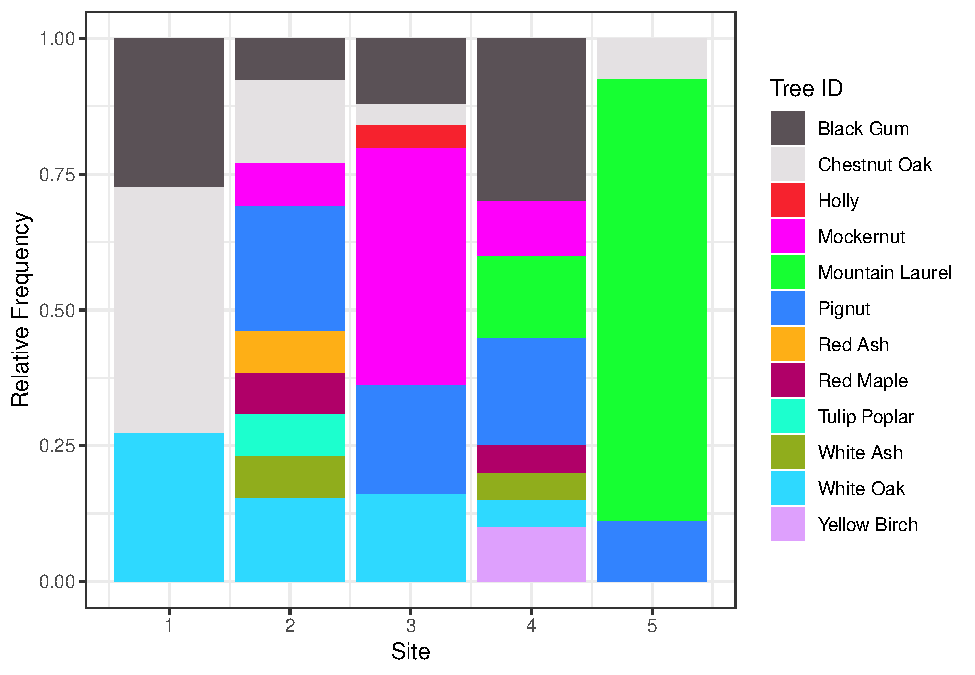
\includegraphics{EVCS-3201_files/figure-latex/unnamed-chunk-13-1.pdf}

\subsection*{Species relative
dominance}\label{species-relative-dominance}
\addcontentsline{toc}{subsection}{Species relative dominance}

\begin{Shaded}
\begin{Highlighting}[]
\CommentTok{# Data processing}
\NormalTok{rel_dom =}\StringTok{ }\NormalTok{forest }\OperatorTok\StringTok{ }
\StringTok{  }
\StringTok{  }\CommentTok{# Select columns we want to plot}
\StringTok{  }\KeywordTok{select}\NormalTok{(Site, }\StringTok{`}\DataTypeTok{Relative Dominance}\StringTok{`}\NormalTok{, }\StringTok{`}\DataTypeTok{Tree ID}\StringTok{`}\NormalTok{) }\OperatorTok\StringTok{ }
\StringTok{  }
\StringTok{  }\CommentTok{# Get distinct values of each row}
\StringTok{  }\KeywordTok{distinct}\NormalTok{()}

\CommentTok{# Plot the data}
\KeywordTok{ggplot}\NormalTok{(}\DataTypeTok{data =}\NormalTok{ rel_dom) }\OperatorTok{+}
\StringTok{  }\KeywordTok{geom_bar}\NormalTok{(}\KeywordTok{aes}\NormalTok{(}\DataTypeTok{x =}\NormalTok{ Site, }\DataTypeTok{y =} \StringTok{`}\DataTypeTok{Relative Dominance}\StringTok{`}\NormalTok{,}
               \DataTypeTok{fill =} \StringTok{`}\DataTypeTok{Tree ID}\StringTok{`}\NormalTok{), }\DataTypeTok{stat =} \StringTok{"identity"}\NormalTok{) }\OperatorTok{+}
\StringTok{  }
\StringTok{  }\CommentTok{#add color palette }
\StringTok{  }\KeywordTok{scale_fill_manual}\NormalTok{(}\DataTypeTok{values =} \KeywordTok{as.vector}\NormalTok{(pals}\OperatorTok{::}\KeywordTok{polychrome}\NormalTok{(}\DecValTok{35}\NormalTok{)))}\OperatorTok{+}
\StringTok{  }\KeywordTok{theme_bw}\NormalTok{()}
\end{Highlighting}
\end{Shaded}

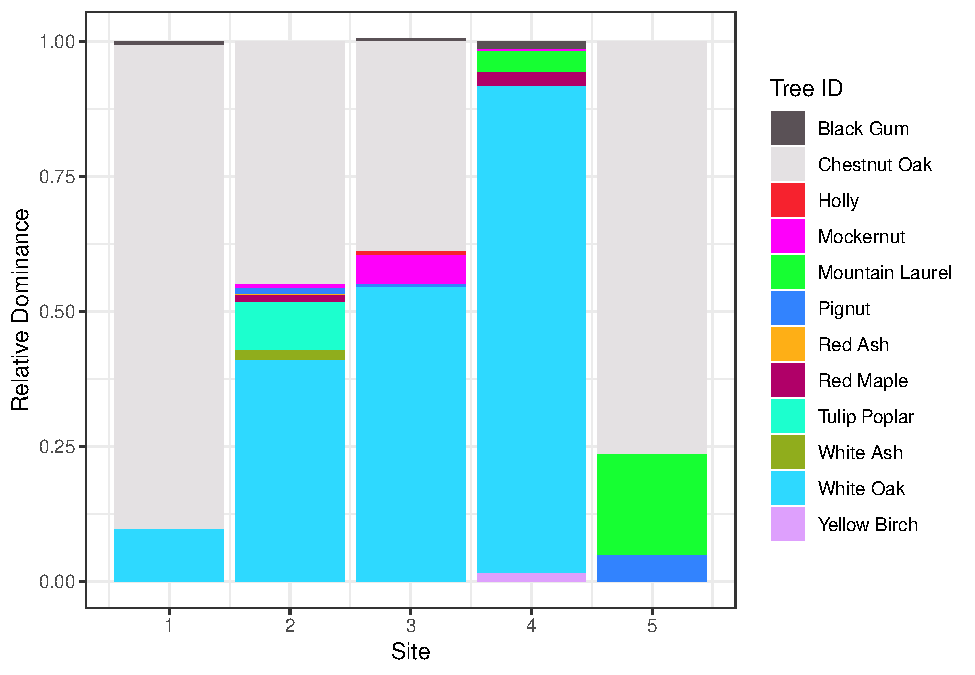
\includegraphics{EVCS-3201_files/figure-latex/unnamed-chunk-14-1.pdf}

\subsection*{Species importance}\label{species-importance}
\addcontentsline{toc}{subsection}{Species importance}

\begin{Shaded}
\begin{Highlighting}[]
\CommentTok{# Data processing}
\NormalTok{importance =}\StringTok{ }\NormalTok{forest }\OperatorTok\StringTok{ }
\StringTok{  }
\StringTok{  }\CommentTok{# Select columns we want to plot}
\StringTok{  }\KeywordTok{select}\NormalTok{(Site, Importance, }\StringTok{`}\DataTypeTok{Tree ID}\StringTok{`}\NormalTok{) }\OperatorTok\StringTok{ }
\StringTok{  }
\StringTok{  }\CommentTok{# Get distinct values of each row}
\StringTok{  }\KeywordTok{distinct}\NormalTok{()}

\CommentTok{# Plot the data}
\KeywordTok{ggplot}\NormalTok{(}\DataTypeTok{data =}\NormalTok{ importance) }\OperatorTok{+}
\StringTok{  }\KeywordTok{geom_bar}\NormalTok{(}\KeywordTok{aes}\NormalTok{(}\DataTypeTok{x =}\NormalTok{ Site, }\DataTypeTok{y =}\NormalTok{ Importance,}
               \DataTypeTok{fill =} \StringTok{`}\DataTypeTok{Tree ID}\StringTok{`}\NormalTok{), }
           \DataTypeTok{position =} \StringTok{"dodge"}\NormalTok{, }\DataTypeTok{stat =} \StringTok{"identity"}\NormalTok{) }\OperatorTok{+}
\StringTok{  }
\StringTok{  }\CommentTok{#add color palette }
\StringTok{  }\KeywordTok{scale_fill_manual}\NormalTok{(}\DataTypeTok{values =} \KeywordTok{as.vector}\NormalTok{(pals}\OperatorTok{::}\KeywordTok{polychrome}\NormalTok{(}\DecValTok{35}\NormalTok{))) }\OperatorTok{+}
\StringTok{  }\KeywordTok{theme_bw}\NormalTok{()}
\end{Highlighting}
\end{Shaded}

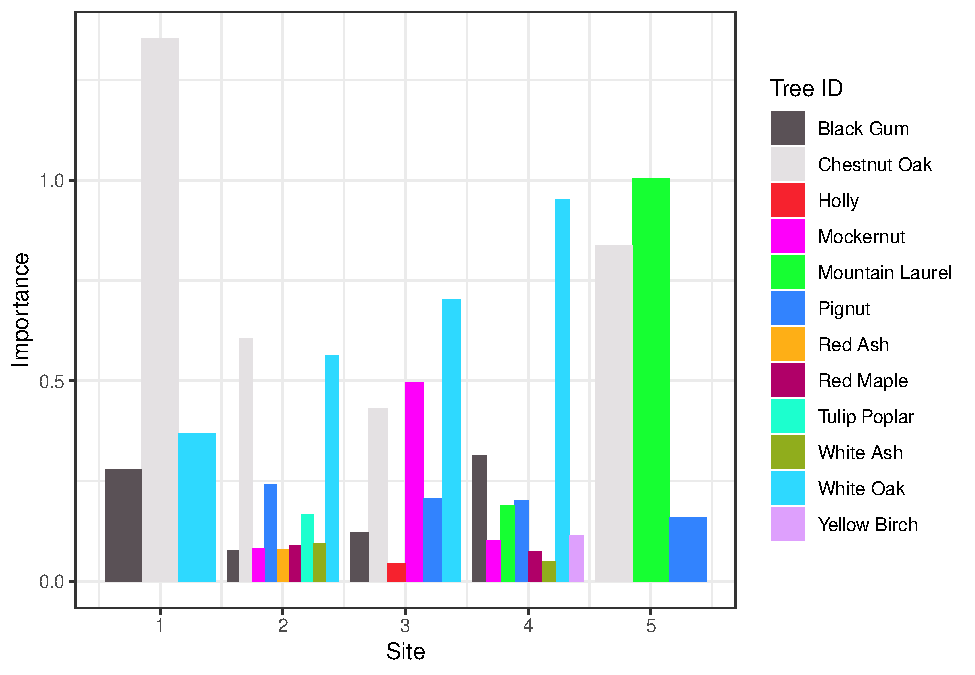
\includegraphics{EVCS-3201_files/figure-latex/unnamed-chunk-15-1.pdf}

\chapter{Stream Lab (week of 3/27)}\label{stream-lab-week-of-327}

\section{Supplemental videos}\label{supplemental-videos}

\subsection*{Stream stressors: impervious
surfaces}\label{stream-stressors-impervious-surfaces}
\addcontentsline{toc}{subsection}{Stream stressors: impervious surfaces}

\href{https://www.youtube.com/embed/wZGzqDfoIks}{
\includegraphics{EVCS-3201_files/figure-latex/unnamed-chunk-16-1.pdf}}

\subsection*{Stream restoration in Baltimore
County}\label{stream-restoration-in-baltimore-county}
\addcontentsline{toc}{subsection}{Stream restoration in Baltimore
County}

\href{https://www.youtube.com/embed/jIGoCM2sCBM}{
\includegraphics{EVCS-3201_files/figure-latex/unnamed-chunk-17-1.pdf}}

\subsection*{Stream characteristics: pools and
riffles}\label{stream-characteristics-pools-and-riffles}
\addcontentsline{toc}{subsection}{Stream characteristics: pools and
riffles}

\href{https://www.youtube.com/embed/RGM1X6rcWEE}{
\includegraphics{EVCS-3201_files/figure-latex/unnamed-chunk-18-1.pdf}}

\section{Discussion questions}\label{discussion-questions}

Video 1. Scientists from the Smithsonian Environmental Research Center
use biodiversity assessments to quantify the health of stream habitats.
How would you expect an increase in nearby impervious surfaces to affect
the \textbf{abundance} and \textbf{biodiversity} of stream
macroinvertebrates? Why?

Video 2. In Northern Virginia, rapid development has led to increased
run-off and subsequent stream erosion. According to the video about
Baltimore County stream restoration, what are two methods that are used
to restore streams in developed areas?

Video 3. Pool and riffle sequences are characterized by unique flow
characteristics. After reading pages 29-35 in the lab manual and
watching the video on pools and riffles, would you expect biodiversity
and abundance to be higher in pools or in riffles? Why?

\section{Assignments}\label{assignments}

Assignments are due on March 29th March 27th by 2 pm.

\begin{enumerate}
\def\labelenumi{\arabic{enumi}.}
\item
  Use this week's reading (pages 29-35 in your lab manual) and the
  embedded videos to answer the discussion questions listed above.
  Submit in a word document.
\item
  Don't forget that forest lab questions and abstract are also due!
\item
  The stream lab involves calculating Simpson's diversity index (D) (lab
  manual pg. 36) and species
  \href{https://en.wikipedia.org/wiki/Rank_abundance_curve}{rank
  abundance curves}. Download the file \texttt{dinosaur\_example.xlsx}
  from collab, and see if you can calculate D and rank abundance from
  the given abundance data ``sampled'' at Site A and Site B. Give it a
  shot over next week and we will finish/discuss it in class.
\end{enumerate}

Here's the Excel calculation for \textbf{Site A}:

\begin{center}\includegraphics{images/dinosaur_example} \end{center}

\chapter{Stream Lab 2 (week of 4/3)}\label{stream-lab-2-week-of-43}

\section{Assignments}\label{assignments-1}

This week's assignment is to complete the introduction and methods
sections for your Stream Lab report. The due date for this assignment is
\textbf{Monday, April 6th at 11:59 PM}.

\begin{itemize}
\tightlist
\item
  Instructions for your assignment are listed on \textbf{page 35} of
  your lab manual.
\item
  Have another look at the lecture powerpoint from last week for
  supplemental information that may be useful for writing.
\end{itemize}

Check back here in a couple of days for more information regarding data
analysis for your Results and Discussion sections; due \textbf{Friday,
April 10th by 2:00 PM}.

\chapter{Stream Lab 3 (week of 4/10)}\label{stream-lab-3-week-of-410}

\section{Hypothesis testing}\label{hypothesis-testing}

The goal of the text and figures below is to describe the \emph{t} test
in a visually intuitive way, and was mostly derived from
\citet{zar1984}. Further information and another example are provided in
your lab manuals on page 36.

\textbf{Hypothesis testing} is all about drawing inferences about a
broader \emph{population} given a \emph{representative sample}. A common
approach to hypothesis testing involves comparing the means of two
samples. For example, consider an experiment where nitrogen fertilizer
was added to the soils of 40 randomly selected plants, with 40 other
plants not recieving the nutrient treatment. The heights of each plant
were measured after two weeks. The results of the experiment are shown
in Figure 4.1.

In this experiment, our null hypothesis (\(H_0\)) is that there is no
difference in mean height between the plants recieving nutrient and
no-nutrient treatments. We can test this hypothesis using a two sample
\emph{t} test, which is designed to infer differences in two populations
being sampled.

\begin{figure}
\centering
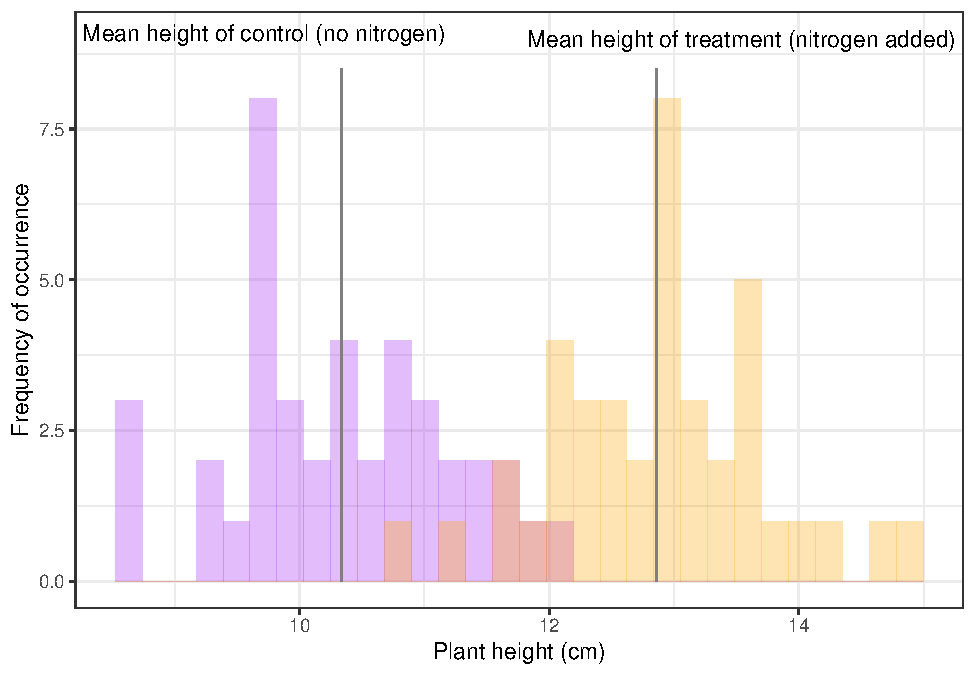
\includegraphics{EVCS-3201_files/figure-latex/compare-1.pdf}
\caption{\label{fig:compare}Histograms showing the heights of two groups of
plants after two weeks of growth. The orange histogram reflects those
plants that recieved a nitrogen treatment and the purple histogram shows
the plants that did not.}
\end{figure}

\subsection{\texorpdfstring{The \emph{t}
statistic}{The t statistic}}\label{the-t-statistic}

Before we jump into the two-sample \emph{t} test, let's explore some
concepts.

First consider the mean height of the no nitrogen sample: 10.3 cm. Next,
say we found a value in the literature suggesting that the mean height
of all plants of this species was 10 cm. Is the mean of this sample
significantly different from the established value?

This leaves us with the null hypothesis \((H_0)\) that there is no
difference between the population mean \((\mu)\) of 10 cm and our sample
mean \((\bar{X})\) of 10.3 cm \((H_0: \mu = \bar{X})\). To test this
hypothesis, we start with the idea that the mean of our sample is only
one of many possible means from samples of size 40 that could have been
drawn at random from the population. Given the population mean of 10 cm
\((\mu = 10\;\textrm{cm})\), we can estimate how unlikely our sample
mean is by calculating a \emph{t} statistic:

\[t = \frac{\bar{X}-\mu}{s_{\bar{X}}} ,\]

where \(\bar{X}\) is the sample mean, \(\mu\) is hypothesized population
mean, and \(s_{\bar{X}}\) is the standard deviation of the sample. If
our sample mean also equals 10, then \(t = 0\). If we resampled the
population a thousand more times, calculated the \emph{t} statistic for
each sample mean, and plotted the histogram of all \emph{t} statistics,
the shape of the histogram would resemble the line in Figure 4.2.

\begin{figure}
\centering
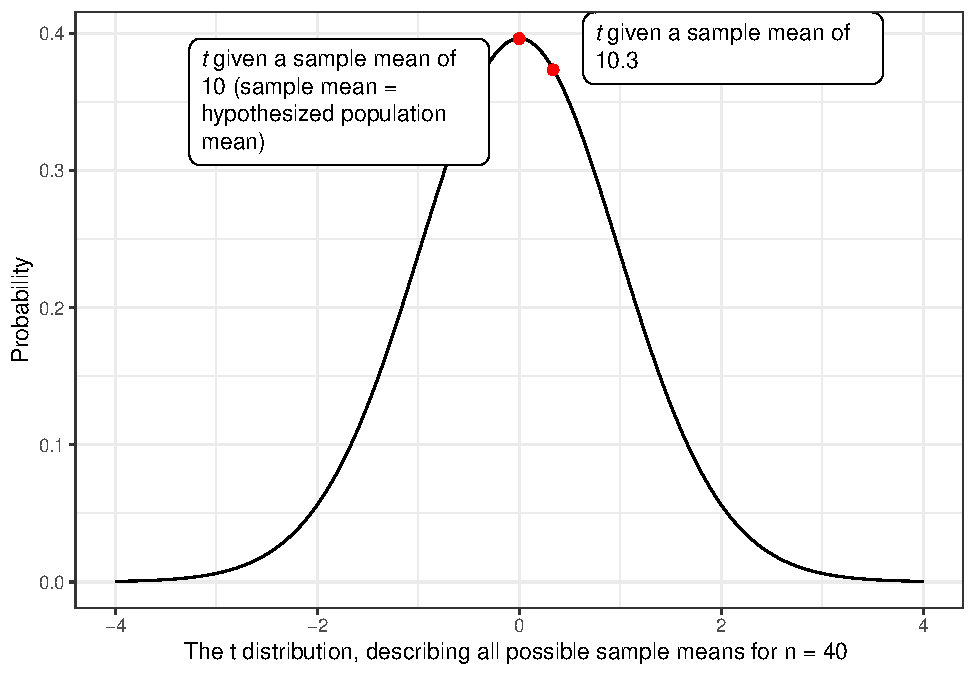
\includegraphics{EVCS-3201_files/figure-latex/unnamed-chunk-21-1.pdf}
\caption{\label{fig:unnamed-chunk-21}The \emph{t} distribution, describing
all possible sample means for n = 40. This \emph{t} distribution is a
\emph{probability distribution}.}
\end{figure}

Figure 4.2 describes the distribution of all possible mean values for a
given sample size, which is known as the \emph{t} distribution. The
shape of the distribution changes according to the \textbf{degrees of
freedom \((v)\)}, which is equal to \(n - 1\). Therefore, our sample has
\(40-1 = 39\) degrees of freedom. As sample size increases, the
``tails'' of the distribution shrink (Fig. 4.3), reflecting a greater
probability of capturing the population mean in your sample.

\begin{figure}
\centering
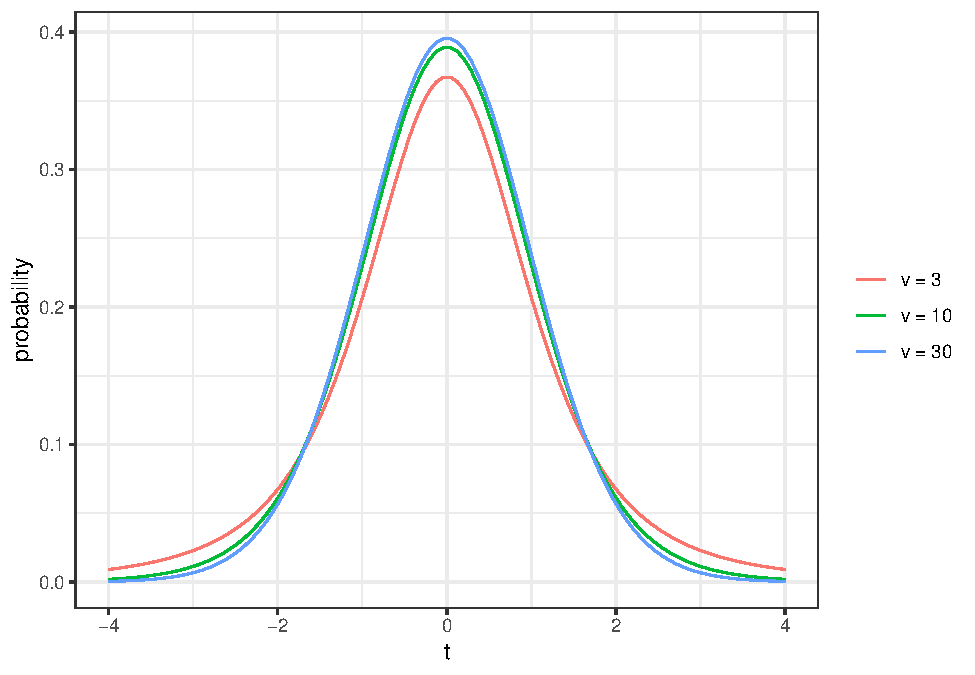
\includegraphics{EVCS-3201_files/figure-latex/unnamed-chunk-22-1.pdf}
\caption{\label{fig:unnamed-chunk-22}The \emph{t} distribution with a range
of degrees of freedom \((v)\). Note how the ``tails'' become larger when
\(v\) is small.}
\end{figure}

Some sample means are more likely than others. In this example, given
the null hypothesis of the population mean being equal to 10
\((H_0: \mu = 10)\), the probability of a sample mean being less than
7.6 cm is less than 2.5\%, and the probability of a sample mean being
greater than 12.4 cm is less than 2.5\%. Therefore, the probability of a
sample mean as extreme or more extreme than either value is less than
5\%, or 0.05 (Fig. 4.4).

\begin{figure}
\centering
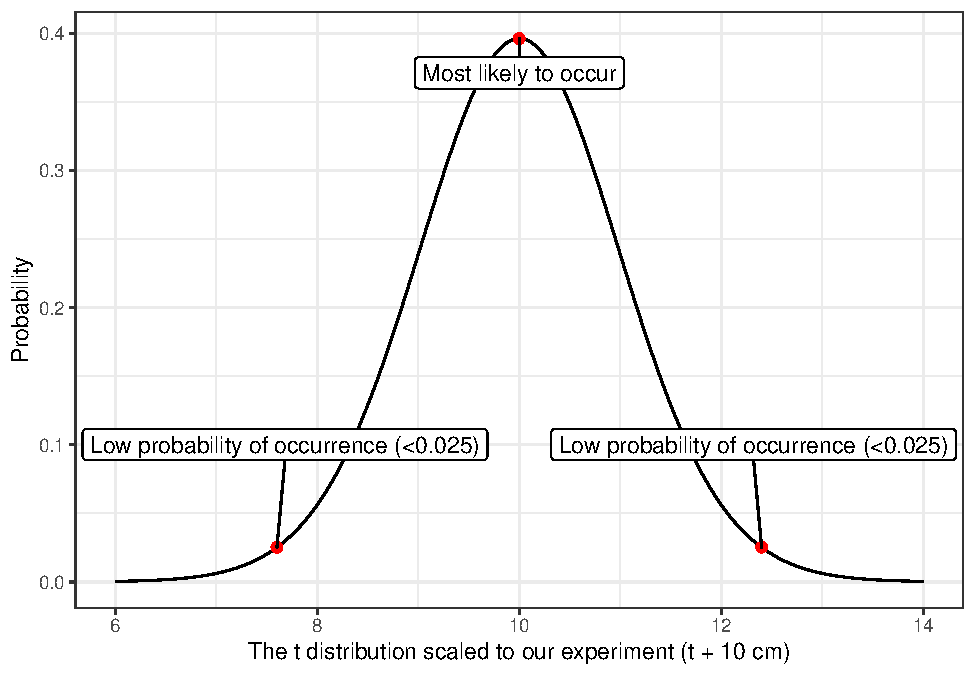
\includegraphics{EVCS-3201_files/figure-latex/unnamed-chunk-23-1.pdf}
\caption{\label{fig:unnamed-chunk-23}The \emph{t} distribution is centered
around \emph{t} = 0. However, we can contextualize the distribution
within our example by adding the hypothesized population mean to
\emph{t} \((t + 10\;\textrm{cm})\).}
\end{figure}

\subsection{\texorpdfstring{The two-sample \emph{t}
test}{The two-sample t test}}\label{the-two-sample-t-test}

It turns out that if two populations have equal variances (the
``spread'' of the data) and are normally distributed, then the ratio of
the difference in means \((\bar{X_1} - \bar{X_2})\) to the standard
error of the difference between the sample means
\((s_{\bar{X_1} - \bar{X_2}})\) is \emph{t} distributed.

The \emph{t} statistic for a two-sample \emph{t} test:

\[t = \frac{\bar{X_1} - \bar{X_2}}{s_{\bar{X_1} - \bar{X_2}}}\]

Therefore, when the above \emph{t} statistic is large, it becomes
unlikely that two samples were drawn from the same population, and it
follows that each \emph{t} statistic is associated with a probability
(\(P\)), just like in our previous example. If \(P\) \textless{} 0.05,
then we can reject the null hypothesis of no difference between the
means of our two samples.

This P value is equivalent to the probability of the \emph{t} statistic
occurring by chance alone upon repeated sampling given that the null
hypothesis is true. When we reject a null hypothesis based on P
\textless{} 0.05 using a two-sample \emph{t} test, it means that the
probability of seeing differences as larger or larger than what we
identified is less than 5\% if the samples were drawn from the same
population.

\subsection{\texorpdfstring{\emph{t} tests in R and
Excel}{t tests in R and Excel}}\label{t-tests-in-r-and-excel}

\subsubsection{R}\label{r}

Here I'll implement the two-sample \emph{t} test as described above for
the plant-nutrient example. In R, two-sample \emph{t} tests are
straightforward once the data are in the correct format.

\begin{Shaded}
\begin{Highlighting}[]
\CommentTok{# first read in data, as practiced in the Forest Lab.}
\NormalTok{df <-}\StringTok{ }\KeywordTok{read.csv}\NormalTok{(}\DataTypeTok{file =} \StringTok{"/users/seanhardison/documents/git/EVSC-3201/data/nutrient_example.csv"}\NormalTok{)}

\CommentTok{# view the first ten rows of data. }
\KeywordTok{head}\NormalTok{(df)}
\end{Highlighting}
\end{Shaded}

\begin{verbatim}
##   no_nitrogen nitrogen_added  X X.1 X.2 X.3 X.4 X.5 X.6 X.7 X.8 X.9 X.10 X.11
## 1    9.338150       12.56883 NA  NA  NA  NA  NA  NA  NA                      
## 2   11.718954       13.38245 NA  NA  NA  NA  NA  NA  NA                      
## 3   12.121667       13.04113 NA  NA  NA  NA  NA  NA  NA                      
## 4   11.497154       12.94078 NA  NA  NA  NA  NA  NA  NA                      
## 5    9.963859       11.70358 NA  NA  NA  NA  NA  NA  NA                      
## 6   11.231945       10.86302 NA  NA  NA  NA  NA  NA  NA
\end{verbatim}

\begin{Shaded}
\begin{Highlighting}[]
\CommentTok{# do the t test comparing means between nutrient treatments}
\KeywordTok{t.test}\NormalTok{(df}\OperatorTok{$}\NormalTok{no_nitrogen, df}\OperatorTok{$}\NormalTok{nitrogen_added)}
\end{Highlighting}
\end{Shaded}

\begin{verbatim}
## 
##  Welch Two Sample t-test
## 
## data:  df$no_nitrogen and df$nitrogen_added
## t = -12.759, df = 77.952, p-value < 2.2e-16
## alternative hypothesis: true difference in means is not equal to 0
## 95 percent confidence interval:
##  -2.920589 -2.132171
## sample estimates:
## mean of x mean of y 
##  10.33504  12.86142
\end{verbatim}

The results show that \(t = -12.79\) and \(P < 0.0001\). Therefore, we
can reject the null hypothesis that there was no effect of nitrogen
treatment, lending support to the alternative hypothesis that nitrogen
is beneficial for plant growth.

\subsubsection{Excel}\label{excel}

The process in Excel is just as quick and easy as in R.

\begin{enumerate}
\def\labelenumi{\arabic{enumi}.}
\tightlist
\item
  Once your spreadsheet is open, select the \textbf{Data Analysis} tab
\item
  Next, select \textbf{t-Test: Two-Sample Assuming Equal Variances}
\item
  Select \textbf{Variable 1 Range} and highlight the first column you
  want to compare
\item
  Select \textbf{Variable 2 Range} and highlight the second column you
  want to compare
\item
  Select \textbf{OK}
\end{enumerate}

\includegraphics{images/t_test_example.gif}

\subsection{What do I report?}\label{what-do-i-report}

When referring to a \emph{t} test in the text, you should report the
\emph{t} statistic, degrees of freedom, and P value.

When presenting results of a \emph{t} test, refer to Table 2 on page 39
of your lab manual.

\subsection{Assignments}\label{assignments-2}

\begin{enumerate}
\def\labelenumi{\arabic{enumi}.}
\tightlist
\item
  This week's assignment is to write the results and discussion sections
  for your stream lab report. Complete instructions are available on
  pages 40-41 of your lab manual. The deadline for this assignment is
  \textbf{Friday, April 10th at 2 PM}.
\end{enumerate}

\bibliography{book.bib,packages.bib}

\end{document}
